\documentclass[12pt]{article}
\usepackage[margin=1in]{geometry}
\usepackage{amsmath,amssymb}
\usepackage{enumerate}
\usepackage{tikz}
\usepackage{xcolor}

\pagestyle{empty}

\begin{document}

\begin{center}
  \textbf{\large Math 3305 --- Exam 1 Practice}
\end{center}

\bigskip

\begin{enumerate}
  \item The GPAs of a sample of 5 students enrolled in Math 3305 are obtained:
    \[
      \{3.2,\; 2.3,\; 3.4,\; 4.0,\; 3.0\}.
    \]
    Find the values of the following statistics. Use the correct symbol for each.
    \begin{enumerate}[(a)]
      \item Sample median.
      \item Sample mean.
      \item Sample standard deviation.
    \end{enumerate}

  \setcounter{enumi}{3}
  \item In the diagram below, A, B, and C are switches that may be closed (current flows through the switch) or open (current cannot flow through the switch). Show the sample space indicating all the possible positions of the switches in the circuit.

    \begin{center}
    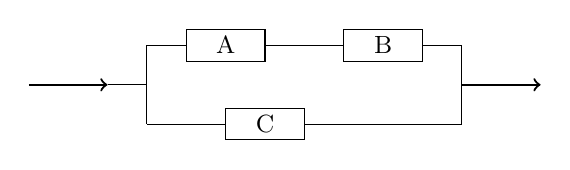
\begin{tikzpicture}[scale=1, every node/.style={font=\small}]
      % left wire
      \draw[->, thick] (-0.5,0.5) -- (0.5,0.5);
      % split
      \draw (0.5,0.5) -- (1,0.5) -- (1,1);
      \draw (1,0.5) -- (1,0);
      % top branch: A and B
      \draw (1,1) -- (1.5,1);
      \draw (1.5,0.8) rectangle (2.5,1.2);
      \node at (2,1) {A};
      \draw (2.5,1) -- (3.5,1);
      \draw (3.5,0.8) rectangle (4.5,1.2);
      \node at (4,1) {B};
      \draw (4.5,1) -- (5,1);
      % bottom branch: C
      \draw (1,0) -- (2,0);
      \draw (2,-0.2) rectangle (3,0.2);
      \node at (2.5,0) {C};
      \draw (3,0) -- (5,0);
      % merge
      \draw (5,1) -- (5,0.5);
      \draw (5,0) -- (5,0.5);
      % right wire
      \draw[->, thick] (5,0.5) -- (6,0.5);
    \end{tikzpicture}
    \end{center}

\newpage

  \setcounter{enumi}{9}
  \item An assembly line is observed until items of both types---good (G) items and items not meeting specification (N)---are observed. Show the sample space.

  \item A candy bar with a 25-gram label weight is selected at random from a production line and weighted. Assuming that a candy bar cannot exceed 25 grams in weight, specify the sample space.

\newpage

  \item Determine whether each sample space in Problems 2--4 above is a countable sample space.

  \item A six-sided die is color-painted on sides (four in red or two in blue) as: \textcolor{red}{1}, \textcolor{red}{2}, \textcolor{red}{3}, \textcolor{blue}{4}, \textcolor{red}{5}, \textcolor{blue}{6}. Roll the die once and observed the side on top. Let $A =$ ``blue'', $B =$ ``min or max'', and $C =$ ``odd''.
    \begin{enumerate}[(a)]
      \item Describe the relationship between $\bar{A}$ and $B$.
      \item Determine the elements of $B \cup C$ and $\bar{B} \cup \bar{C}$.
    \end{enumerate}

\newpage

  \item A manufacturer of pickup trucks is required to recall all the trucks manufactured in a given year for the repair of possible defects in the steering column and defects in the brake linings. Dealers have been notified that 3\% of the trucks have defective steering, and that 4\% of the trucks have defective brake linings. If 94\% of the trucks have neither defect, what percentage of the trucks have both defects?

  \item \begin{enumerate}[(a)]
      \item Explain why $P(A \cup B) \leq P(A) + P(B)$.
      \item Explain why $P(A \cup B \cup C) \leq P(A) + P(B) + P(C)$.
    \end{enumerate}

\newpage

  \item Toss a fair coin three times and observe the result.
    \begin{enumerate}[(a)]
      \item Determine the sample space.
      \item Let $A =$ ``at most one heads'', $B =$ ``at least one heads'', and $C =$ ``heads on the second toss''. Find $P(A)$, $P(\bar{B})$, $P(A \cap B)$, and $P(A \cup C)$.
    \end{enumerate}

  \item If $P(A) = 0.6$, $P(B) = 0.5$, $P(A \cap B) = 0.4$, find $P(A \cup B)$ and $P(\bar{A} \cup \bar{B})$.

\newpage

  \item In a small school, 5 centers, 7 guards, and 6 forwards try out for the basketball team, which has one center, two guards, and two forwards. How many five-member teams can be formed from these players?

  \item In how many different ways can the letters in the word ``correspondences'' be arranged?

\newpage

  \item A small pond contains 40 fish, 10 of which have been tagged. If a catch of 7 fish is made, in how many ways can the catch contain exactly 2 tagged fish?

  \item A shipment of 15 components will be accepted by a buyer if a random sample of 3 (chosen without replacement) contains no defectives. What is the probability the shipment will be rejected if actually 2 of the components are defective?

\newpage

  \item In a sample space, events $A$ and $B$ are independent; events $B$ and $C$ are mutually exclusive, and $A$ and $C$ are independent. If $P(A \cup B \cup C) = 0.9$ while $P(B) = 0.5$ and $P(C) = 0.3$, find $P(A)$.

  \item If $P(A \cup B) = 0.4$ and $P(A) = 0.3$, find $P(B)$ if
    \begin{enumerate}[(a)]
      \item $A$ and $B$ are independent.
      \item $A$ and $B$ are mutually exclusive.
    \end{enumerate}

\newpage

  \item A coin, loaded so that the probability it shows heads when tossed is $3/4$, is tossed twice. Let the events $A$, $B$, and $C$, be ``first toss is heads,'' ``second toss is heads,'' and ``tosses show the same face,'' respectively.
    \begin{enumerate}[(a)]
      \item Are the events $A$ and $B$ independent?
      \item Are the events $A$ and $B \cup C$ independent?
      \item Are the events $A$, $B$, and $C$ independent?
    \end{enumerate}

  \item A student takes a driving test until it is passed. If the probability the test is passed on any attempt is $4/7$ and if the attempts are independent, what is the probability the test is taken an even number of times?

\newpage

  \item A group of 200 people are classified as follows. A person is randomly selected from this group. Find the following probabilities.

    \begin{center}
    \begin{tabular}{l|cccc}
               & \multicolumn{4}{c}{\textbf{Blood Type}} \\
      \textbf{Gender} & O & A & B & AB \\ \hline
      Male     & 36 & 20 & 28 & 16 \\
      Female   & 40 & 30 & 20 & 10 \\
    \end{tabular}
    \end{center}

    \begin{enumerate}[(a)]
      \item A person with type O blood is selected.
      \item The selected person is either a female or has type O blood.
      \item A male with type B blood is selected.
      \item The selected person is female if the person has type O blood.
    \end{enumerate}

  \item An urn contains eight balls labeled $1, 2, \dots, 8$. One ball is drawn at random. Define events $A = \{1,2,3,4\}$, $B = \{1,2,5,6\}$, and $D = \{1,3,5,7\}$. Are $A$, $B$, and $D$ mutually independent? Justify.

\newpage

  \item The following model is sometimes used to model the spread of a contagious disease. Suppose a box contains $b$ black and $r$ red marbles. A marble is drawn and $c$ marbles of that color together with the drawn marble are replaced in the box before the next marble is drawn, so that infected persons infect others while immunity to the disease may also increase.
    \begin{enumerate}[(a)]
      \item Find the probability that the first three marbles drawn are red.
      \item Show that the probability of drawing a black on the second draw is the same as the probability of drawing a black on the first draw.
      \item Show by induction that the probability the $k$th marble is black is the same as the probability of drawing a black on the first draw.
    \end{enumerate}

  \item Find the reliability of the system below if each component has reliability $0.92$.

    \begin{center}
    \begin{tikzpicture}[scale=1.2, every node/.style={font=\small}]
      % nodes
      \coordinate (L) at (0,0);
      \coordinate (TM) at (2,1.2);
      \coordinate (BM) at (2,-1.2);
      \coordinate (R) at (4,0);
      % input/output arrows
      \draw[->, thick] (-1,0) -- (L);
      \draw[->, thick] (R) -- (5,0);
      % top path: A then B
      \draw (L) -- (TM) node[midway, above left] {$A$};
      \draw (TM) -- (R) node[midway, above right] {$B$};
      % bottom path: D then C
      \draw (L) -- (BM) node[midway, below left] {$D$};
      \draw (BM) -- (R) node[midway, below right] {$C$};
      % bridge: E
      \draw (TM) -- (BM) node[midway, right] {$E$};
    \end{tikzpicture}
    \end{center}

\newpage

  \item \begin{enumerate}[(a)]
      \item There is a fifty-fifty chance that firm A will bid for the construction of a bridge. Firm B submits a bid and the probability that it will get the job is $2/3$, provided firm A does not bid; if firm A submits a bid, the probability firm B gets the job is $1/5$. Firm B is awarded the job; what is the probability firm A did not bid?
      \item In part (a), suppose now that the probability firm B gets the job if firm A bids on the job is $p$. Graph the probability that firm A did not bid given that B gets the job as a function of~$p$.
      \item Generalize parts (a) and (b) further and suppose that the probability that B gets the job given that firm A bids on the job is $r$. Graph the surface showing the probability firm A did not bid, given that firm B gets the job as a function of $p$ and~$r$.
    \end{enumerate}

  \item Three distinct methods, A, B, and C, are available for teaching a certain industrial skill. The failure rates are 30\%, 20\%, and 10\%, respectively. However, due to costs, A is used twice as frequently as B, which is used twice as frequently as C.
    \begin{enumerate}[(a)]
      \item What is the overall failure rate in teaching the skill?
      \item A worker is taught the skill, but fails to learn it correctly. What is the probability he was taught by method~A?
    \end{enumerate}

\newpage

  \item A lie detector is accurate $3/4$ of the time. That is, if a person is telling the truth, the lie detector indicates he is telling the truth with probability $3/4$ while if the person is lying, the lie detector indicates that he is lying with probability $3/4$. Assume that a person taking the lie detector test is unable to influence its results and also assume that 95\% of the people taking the test tell the truth. What is the probability that a person is lying if the lie detector indicates that he is lying?
\end{enumerate}

\end{document}
